\subsection{Vægtede grafer}
En vægtet graf er en graf, hvori kanterne eller knuderne får tildelt en numerisk værdi. I dette projekt arbejdes der udelukkende med vægtede kanter, og vi vil derfor kun fokusere på dem i dette afsnit.
En vægtet graf er defineret ved:
\begin{defn}[Vægtede grafer]
En vægtet graf, $G=(V,E,w)$, består af mængden af knuder, $V$, mængden af kanter, $E \subseteq \{\{u;v\}|u,v \in V\}$, og vægtfunktionen, $w: E \rightarrow \R$.
\end{defn}


For en vægtet graf har alle kanter $e\in E$ en numerisk vægt, givet ved funktionen $w (e)$. Da $e$ er en kant incident med $\{u,v\}$ kan man  ligeledes skrive $w (u,v)$.
\begin{figure}[H]
\centering
	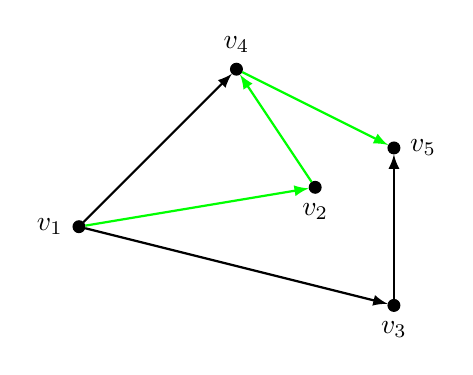
\begin{tikzpicture}

      \tikzset{enclosed/.style={draw, circle, inner sep=0pt, minimum size=.15cm, fill=black}}
%% Vertices
      	\node[enclosed, label={left: $v_1$}] (v1) at (0,2) {};
      	\node[enclosed, label={below: $v_2$}] (v2) at (3,2.5) {};
    		\node[enclosed, label={below: $v_3$}] (v3) at (4,1) {};
  	    \node[enclosed, label={above: $v_4$}] (v4) at (2,4) {};
     	\node[enclosed, label={right: $v_5$}] (v5) at (4,3) {};
%Edges
		\path [->, >=latex, thick, green](v1) edge node[midway, sloped, above] {} (v2);
		\path [->, >=latex, thick](v1) edge node[midway, sloped, above] {} (v3);
		\path [->, >=latex, thick](v1) edge node[midway, above] {} (v4);
		\path [->, >=latex, thick, green](v2) edge node[near end, sloped, below] {} (v4);
		\path [->, >=latex, thick](v3) edge node[midway, below] {} (v5);
		\path [->, >=latex, thick, green](v4) edge node[near end, sloped, above] {} (v5);

	\end{tikzpicture}
	\caption{Eksempel på en orienteret simpel graf og en vej fra $v_{0}$ til $v_{4}$}
	\label{fig.vaegtetopg}
\end{figure}

Da vægtede grafer har en numerisk vægt på hver kant, kan man således beregne længden fra en knude til en anden i grafen. Længden fra en knude til en anden kan defineres således:

\begin{defn}
Lad $m\in \N $ og $G=(V,E,w)$ være en simpel graf og lad $e_{i,i+1}$ være en kant incident med $i$ og $i+1$. Lad en tilfældig vej, $P$, gå gennem knuderne således $P=(v_0,v_1...v_m)$, da kan længden beskrives således:
	\begin{equation*}
	dist(P)=\sum_{i=1}^{m}w(e_{i,i+1})
	\end{equation*}  
\end{defn}

Man kan således bruge følgende definitioner af korteste og længste vej i en vægtet graf:


\begin{defn} [Korteste vej i vægtet graf]\label{defn:min.vej}
Lad $G=(V,E,w)$ være en simpel og vægtet graf. Da er længden af den korteste vej, fra en knude, $v_0$, til en anden knude, $v_m$, defineret som $\alpha(v_0,v_m)$.
\end{defn}

På samme vis defineres længste vej:

\begin{defn} [Længste vej i en vægtet graf]
Lad $G=(V,E,w)$ være en simpel og vægtet graf. Da er længden af den længste vej, fra en knude, $v_0$, til en anden knude, $v_m$, defineret som $\beta(v_0,v_m)$.
\end{defn}

\begin{exmp}
Betragt figur \ref{fig.vaegtetopg} \\
\begin{figure}[H]
\centering
	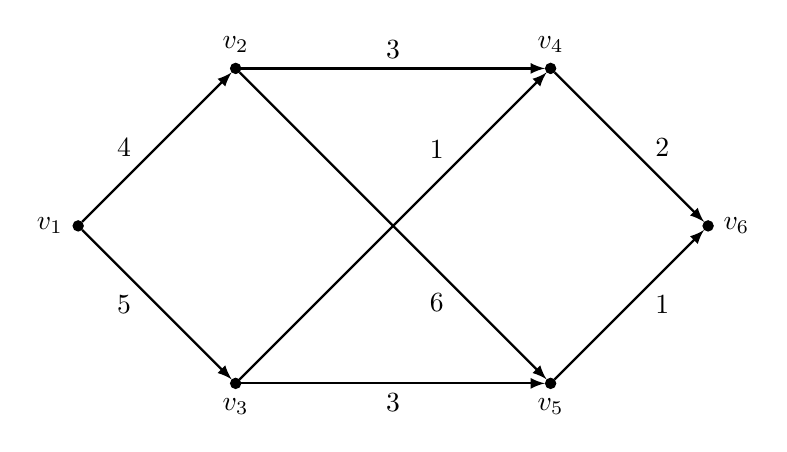
\begin{tikzpicture}

      \tikzset{enclosed/.style={draw, circle, inner sep=0pt, minimum size=.13cm, fill=black}}
%% Vertices
      	\node[enclosed, label={left: $v_1$}] (v1) at (0,2) {};
      	\node[enclosed, label={above: $v_2$}] (v2) at (2,4) {};
    	\node[enclosed, label={below: $v_3$}] (v3) at (2,0) {};
  	    \node[enclosed, label={above: $v_4$}] (v4) at (6,4) {};
     	\node[enclosed, label={below: $v_5$}] (v5) at (6,0) {};
     	\node[enclosed, label={right: $v_6$}] (v6) at (8,2) {};
%Edges
		\path [->, > = latex, thick] (v1) edge node[midway, left=2mm] {4} (v2);
		\path [->, > = latex, thick] (v1) edge node[midway, left=2mm] {$ 5 $} (v3);
		\path [->, > = latex, thick] (v2) edge node[midway, above] {$ 3 $} (v4);
		\path [->, > = latex, thick] (v2) edge node[near end, left=2mm] {$ 6 $} (v5);
		\path [->, > = latex, thick] (v3) edge node[midway, below] {$ 3 $} (v5);
		\path [->, > = latex, thick] (v3) edge node[near end, left=2mm] {$ 1 $} (v4);
		\path [->, > = latex, thick] (v4) edge node[midway, right=2mm] {$ 2 $} (v6);
		\path [->, > = latex, thick] (v5) edge node[midway, right=2mm] {$ 1 $} (v6);

	\end{tikzpicture}
	\caption{Orienteret, simpel og vægtet graf.}
	\label{fig.vaegtetopg}
\end{figure}


På figuren ses en graf med vægtede kanter. Vi er interesserede i at finde den korteste vej fra $v_1$ til $v_6$. For at finde den korteste vej, kigger vi på alle de mulige veje fra $v_1$ til $v_6$.
Følgende veje ses:
\begin{align*}
	P_1=&(v_1,v_2,v_4,v_6)\\
	P_2=&(v_1,v_2,v_5,v_6)\\
	P_3=&(v_1,v_3,v_5,v_6)\\
	P_4=&(v_1,v_3,v_4,v_6)
\end{align*}
Man kan nu beregne længden af de fire veje, ved at tage summen af de kanter, vejen følger. Man får derved:
\begin{align*}
	P_1=&4+3+2=9\\
	P_2=&4+6+1=11\\
	P_3=&5+3+1=9\\
	P_4=&5+1+2=8
\end{align*}
Det ses, at den korteste vej fra $v_1$ til $v_6$ er $P_4$. 
Det er sådan, man kan finde korteste vej i en vægtet graf. Dog kan denne metode blive meget tidskrævende ved mere komplekse grafer. I disse tilfælde vil man bruge alternative, bedre algoritmer til at løse problemet. Dette vil vi komme ind på senere i kapitel \ref{kap.algo}.
\end{exmp}
